% Options for packages loaded elsewhere
\PassOptionsToPackage{unicode}{hyperref}
\PassOptionsToPackage{hyphens}{url}
%
\documentclass[
]{article}
\usepackage{amsmath,amssymb}
\usepackage{iftex}
\ifPDFTeX
  \usepackage[T1]{fontenc}
  \usepackage[utf8]{inputenc}
  \usepackage{textcomp} % provide euro and other symbols
\else % if luatex or xetex
  \usepackage{unicode-math} % this also loads fontspec
  \defaultfontfeatures{Scale=MatchLowercase}
  \defaultfontfeatures[\rmfamily]{Ligatures=TeX,Scale=1}
\fi
\usepackage{lmodern}
\ifPDFTeX\else
  % xetex/luatex font selection
\fi
% Use upquote if available, for straight quotes in verbatim environments
\IfFileExists{upquote.sty}{\usepackage{upquote}}{}
\IfFileExists{microtype.sty}{% use microtype if available
  \usepackage[]{microtype}
  \UseMicrotypeSet[protrusion]{basicmath} % disable protrusion for tt fonts
}{}
\makeatletter
\@ifundefined{KOMAClassName}{% if non-KOMA class
  \IfFileExists{parskip.sty}{%
    \usepackage{parskip}
  }{% else
    \setlength{\parindent}{0pt}
    \setlength{\parskip}{6pt plus 2pt minus 1pt}}
}{% if KOMA class
  \KOMAoptions{parskip=half}}
\makeatother
\usepackage{xcolor}
\usepackage[margin=1in]{geometry}
\usepackage{graphicx}
\makeatletter
\newsavebox\pandoc@box
\newcommand*\pandocbounded[1]{% scales image to fit in text height/width
  \sbox\pandoc@box{#1}%
  \Gscale@div\@tempa{\textheight}{\dimexpr\ht\pandoc@box+\dp\pandoc@box\relax}%
  \Gscale@div\@tempb{\linewidth}{\wd\pandoc@box}%
  \ifdim\@tempb\p@<\@tempa\p@\let\@tempa\@tempb\fi% select the smaller of both
  \ifdim\@tempa\p@<\p@\scalebox{\@tempa}{\usebox\pandoc@box}%
  \else\usebox{\pandoc@box}%
  \fi%
}
% Set default figure placement to htbp
\def\fps@figure{htbp}
\makeatother
\setlength{\emergencystretch}{3em} % prevent overfull lines
\providecommand{\tightlist}{%
  \setlength{\itemsep}{0pt}\setlength{\parskip}{0pt}}
\setcounter{secnumdepth}{-\maxdimen} % remove section numbering
\usepackage{bookmark}
\IfFileExists{xurl.sty}{\usepackage{xurl}}{} % add URL line breaks if available
\urlstyle{same}
\hypersetup{
  pdftitle={Reporte de Fecundidad y Maternidad en Chile},
  pdfauthor={Generado por Fec-Mat CL},
  hidelinks,
  pdfcreator={LaTeX via pandoc}}

\title{Reporte de Fecundidad y Maternidad en Chile}
\author{Generado por Fec-Mat CL}
\date{21 de junio de 2025}

\begin{document}
\maketitle

\pandocbounded{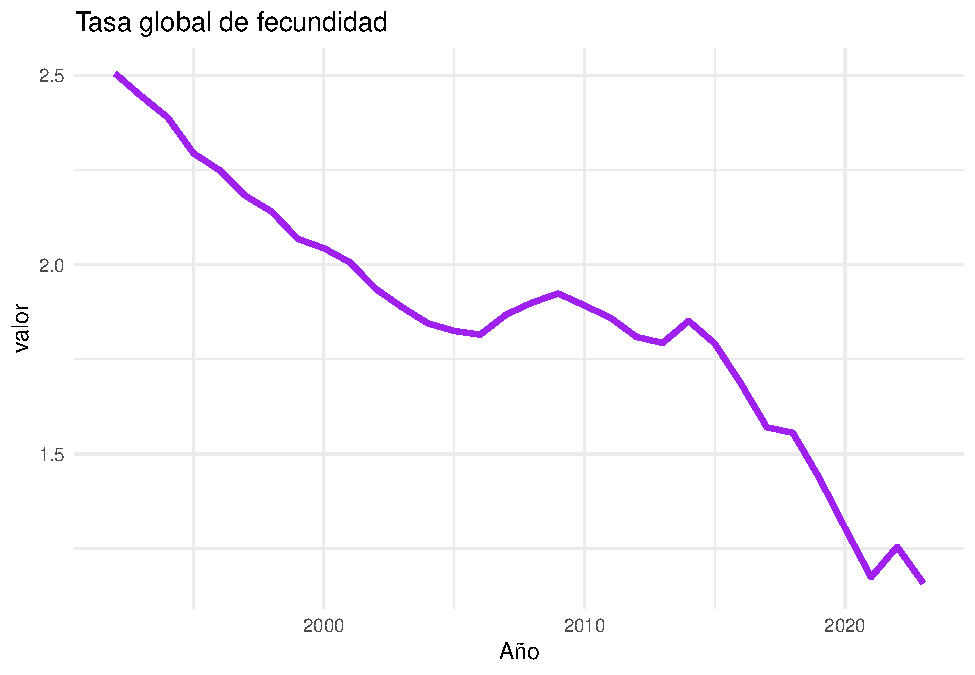
\includegraphics[keepaspectratio]{figs_pdf/errorrrr-1.pdf}}

Entre 1992 y 2023, la \textbf{Tasa Global de Fecundidad (TGF)}
experimentó una disminución, pasando de 2.505 a 1.159. Esta variación
puede considerarse considerablemente desde una perspectiva demográfica.

Una TGF de 1.159 indica que, en promedio, una mujer tendría 1 hijos
durante su vida fértil si se mantuvieran las tasas actuales. Este valor
está por debajo del umbral de reemplazo generacional, lo que sugiere una
tendencia hacia el envejecimiento poblacional y una posible reducción
futura de la población si no existen flujos migratorios compensatorios.

\pandocbounded{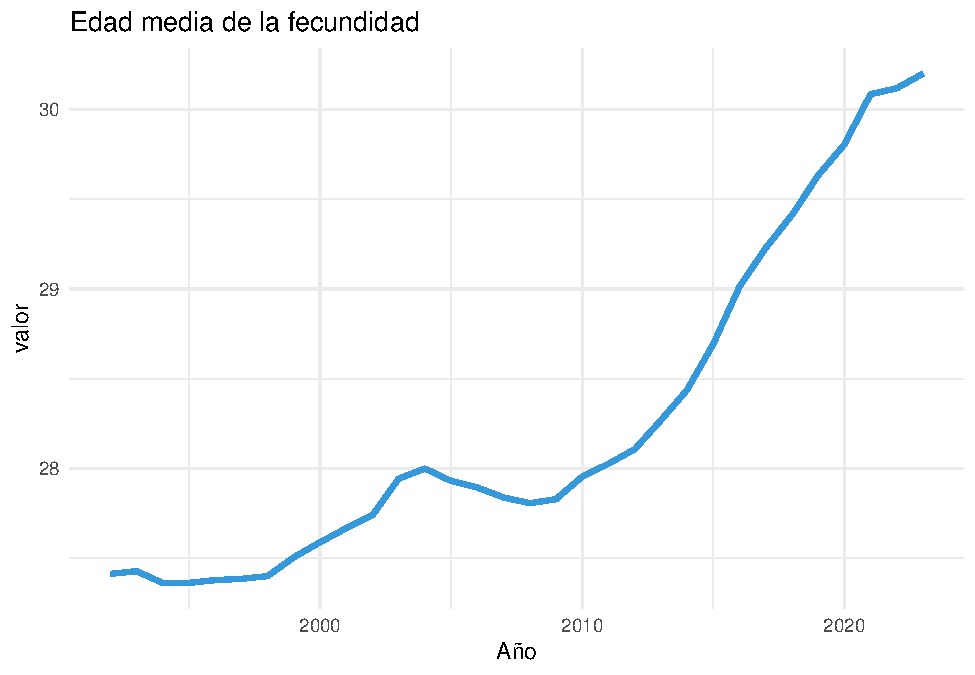
\includegraphics[keepaspectratio]{figs_pdf/grafico_emf-1.pdf}}
Entre 1992 y 2023, la \textbf{Edad Media de la Fecundidad} ha aumentado
en 2.79 años, pasando de 27.4121613590153 a 30.2 años. Este incremento
sugiere una postergación del inicio de la maternidad, posiblemente
asociada a factores como el aumento en la participación laboral
femenina, mayores niveles educativos, cambios culturales y/o condiciones
económicas que incentivan la planificación familiar en edades más
avanzadas. Cabe destacar que este análisis es de carácter descriptivo y
no implica una relación causal. Para confirmar estos patrones, se
requiere un análisis más exhaustivo mediante técnicas inferenciales o
multivariadas apropiadas.

\pandocbounded{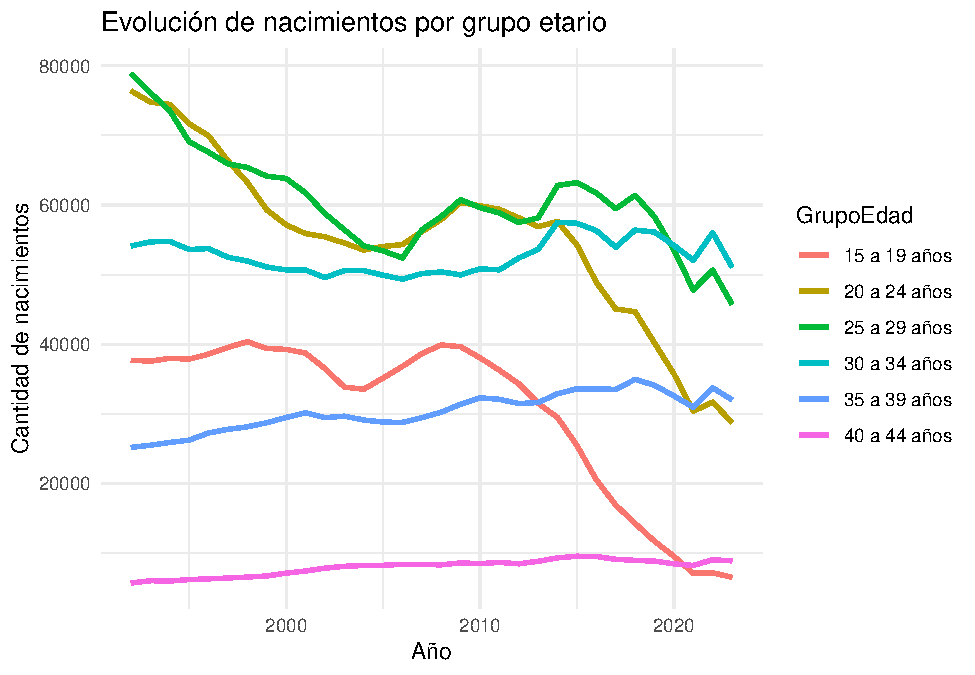
\includegraphics[keepaspectratio]{figs_pdf/nacimiento_prin-1.pdf}}

\textbf{Interpretación automática:} El gráfico muestra la evolución de
los nacimientos anuales en Chile según grupo etario de la madre, para
los rangos entre \textbf{15 y 44 años}. Entre 1992 y 2023, el número
total de nacimientos en estos grupos disminuyó en 104942 nacimientos. El
grupo con mayor descenso fue el de mujeres de \textbf{20 a 24 años}, con
una reducción de 47648 nacimientos. Por otro lado, el grupo de
\textbf{35 a 39 años} registró el mayor incremento, con 6852 nacimientos
adicionales.

\pandocbounded{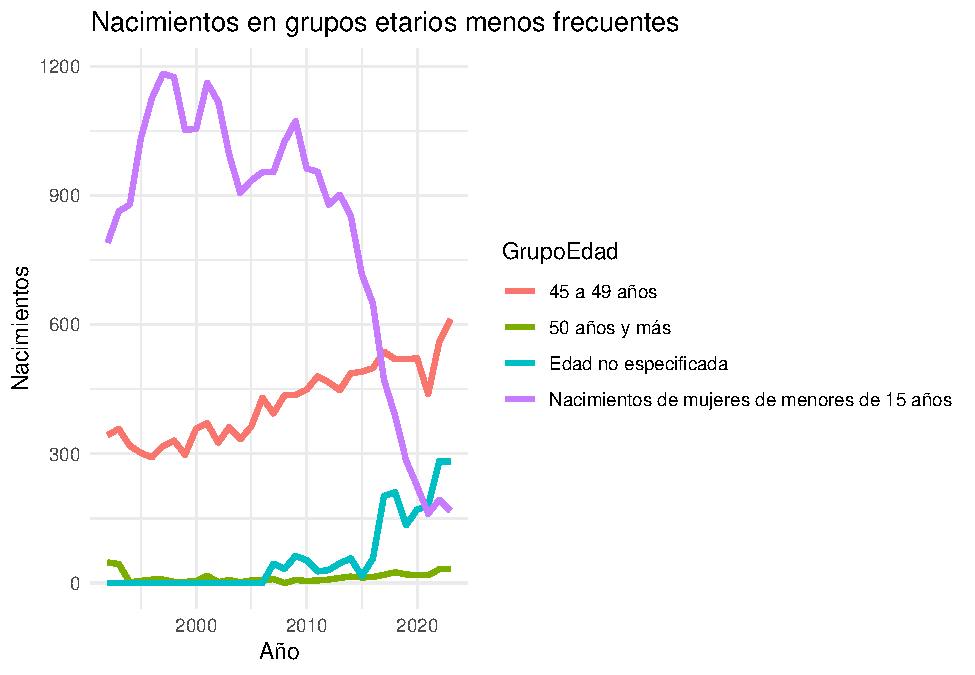
\includegraphics[keepaspectratio]{figs_pdf/nacimiento menores-1.pdf}}

\textbf{Interpretación automática:} El gráfico muestra la evolución de
los nacimientos anuales en Chile para grupos etarios menos frecuentes,
como mujeres menores de 15 años, mayores de 45 y casos con edad no
especificada. El grupo \textbf{45 a 49 años} presentó un aumento de 268
nacimientos entre 1992 y 2023. El grupo \textbf{50 años y más} presentó
un descenso de 16 nacimientos entre 1992 y 2023. El grupo \textbf{Edad
no especificada} presentó un aumento de 282 nacimientos entre 1992 y
2023. El grupo \textbf{Nacimientos de mujeres de menores de 15 años}
presentó un descenso de 623 nacimientos entre 1992 y 2023.

\pandocbounded{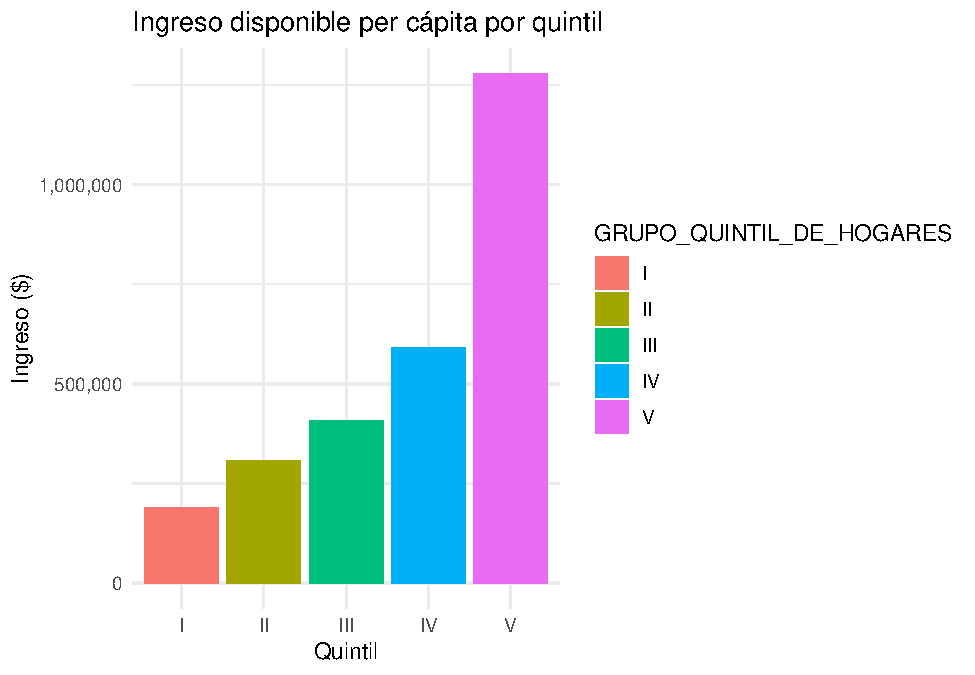
\includegraphics[keepaspectratio]{figs_pdf/quintil-1.pdf}}

\textbf{Interpretación automática:} Se observa una marcada desigualdad
en los ingresos per cápita entre los quintiles. El grupo con menor
ingreso es el quintil I, con un promedio de \$190.432, mientras que el
más alto corresponde al quintil V, con \$1.278.988. Esto implica que el
ingreso promedio del quintil superior es aproximadamente 6.7 veces mayor
al del quintil inferior, evidenciando una brecha significativa que puede
influir en las decisiones de planificación familiar y bienestar general
del hogar.

\pandocbounded{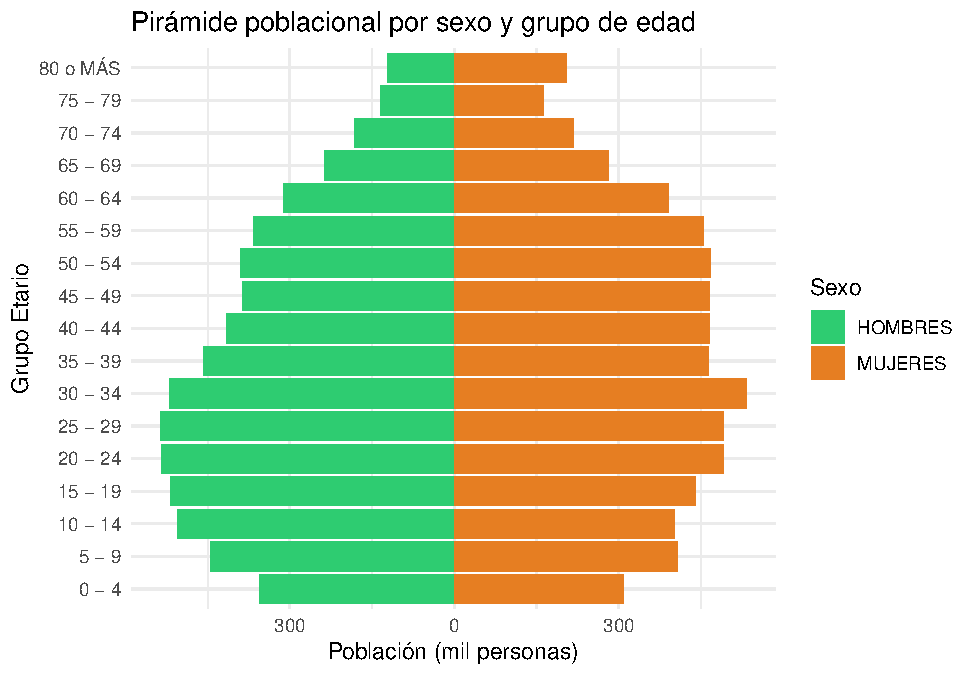
\includegraphics[keepaspectratio]{figs_pdf/piramide-1.pdf}}

\textbf{Interpretación automática:} La pirámide poblacional muestra una
estructura relativamente joven, con un 17.2\% de la población
concentrado en grupos etarios de 60 años o más. El grupo etario más
numeroso corresponde a `30 - 34'. En cuanto a distribución por sexo, se
observa un total de aproximadamente 6.415 mil hombres y 6.649 mil
mujeres, lo cual evidencia una ligera mayoría femenina. Esta composición
etaria y de género puede tener implicancias significativas en la
fecundidad y en la planificación de políticas públicas relacionadas con
salud, educación y seguridad social.

\pandocbounded{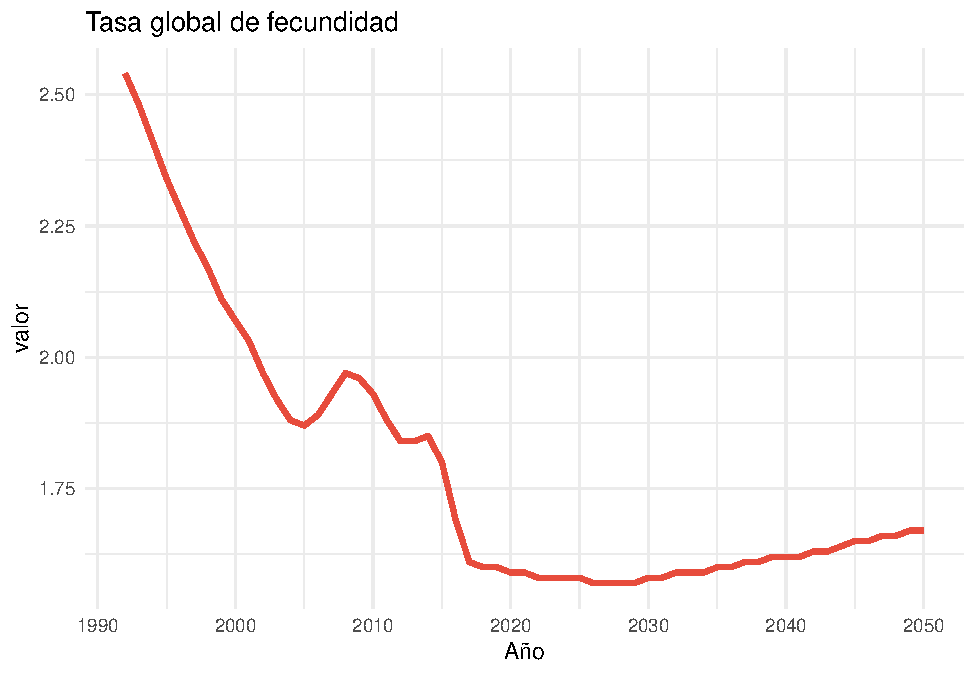
\includegraphics[keepaspectratio]{figs_pdf/grafico_tgf-1.pdf}}

\textbf{Análisis descriptivo de la Tasa Global de Fecundidad (TGF):}
Entre 1992 y 2050, la TGF evidenció un cambio considerable, al pasar de
2.54 a 1.67 hijos por mujer. Este comportamiento representa una
disminución acumulado de 0.87 puntos en el período considerado. Este
indicador resume el promedio de hijos por mujer y su evolución temporal
es clave para entender los cambios estructurales en la dinámica
demográfica del país. Aunque no se infieren causas específicas desde
este análisis, el comportamiento observado puede tener implicancias
relevantes en áreas como planificación social, diseño de políticas
públicas y proyecciones de demanda de servicios en el mediano y largo
plazo.

\pandocbounded{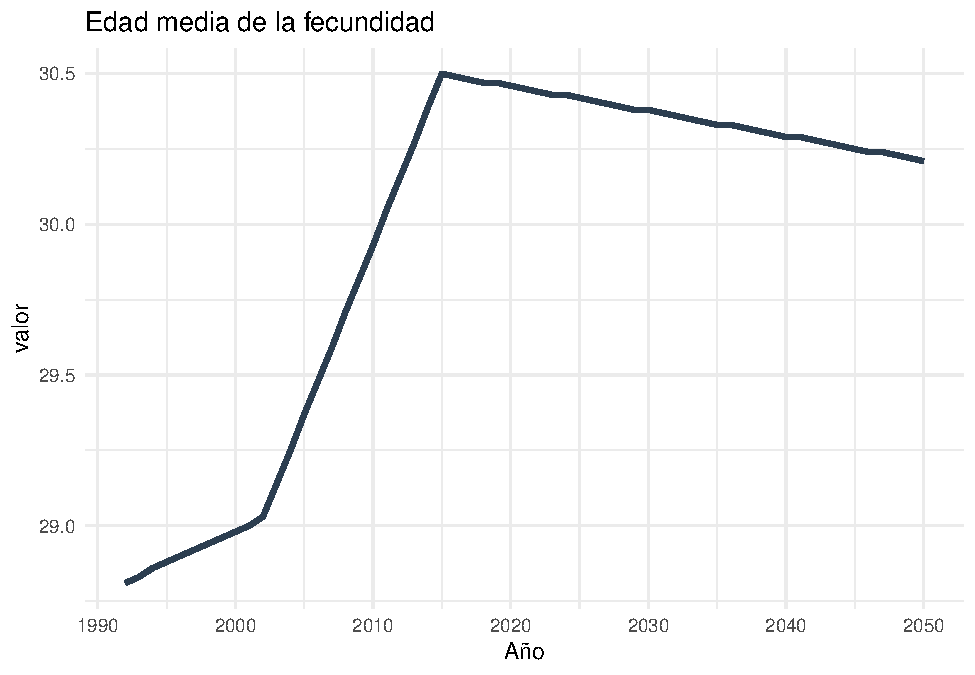
\includegraphics[keepaspectratio]{figs_pdf/grafico_tef-1.pdf}}

\textbf{Edad media de la fecundidad (1992--2050)}: De acuerdo con las
proyecciones oficiales elaboradas a partir del Censo 2017, la edad media
en que las mujeres tienen hijos ha pasado de 28.8 años en 1992 a 30.2
años en 2050, lo que representa un aumento de 1.4 años. Este resultado
entrega una visión resumida sobre cómo ha evolucionado este indicador en
el tiempo reciente,

\pandocbounded{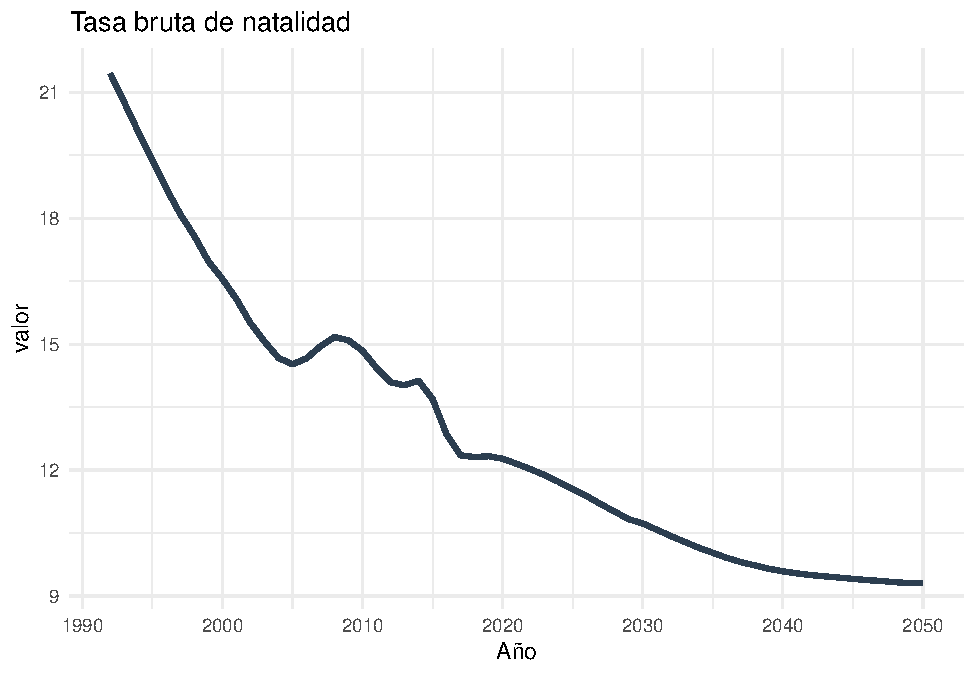
\includegraphics[keepaspectratio]{figs_pdf/grafico_tbn-1.pdf}}

\textbf{Interpretación automática:} Según las proyecciones del INE, la
Tasa Bruta de Natalidad experimentará pronunciada una disminución entre
1992 y 2050, pasando de 21.4 a 9.3 nacimientos por cada 1.000
habitantes. Esta disminución proyectada se alinea con la tendencia de
envejecimiento poblacional y menores tasas de fecundidad observadas en
las últimas décadas.`

\pandocbounded{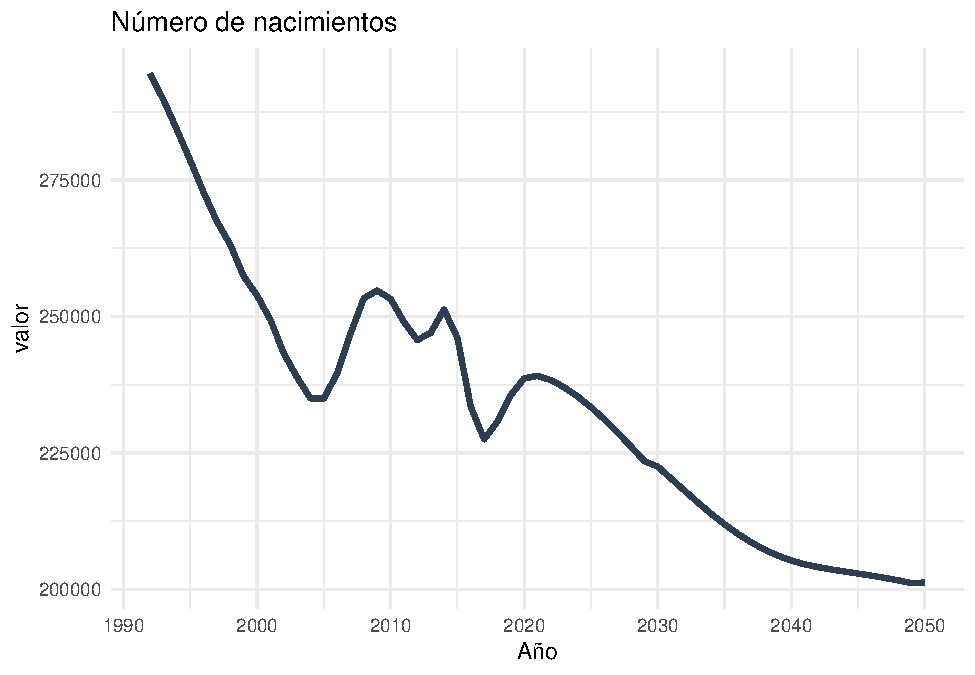
\includegraphics[keepaspectratio]{figs_pdf/nacimientos-1.pdf}}

\textbf{Análisis descriptivo del Número de Nacimientos:} Entre 1992 y
2050, el total anual de nacimientos evidenció un cambio considerable,
pasando de 294,463 a 201,302 nacimientos. Esto representa una
disminución absoluta de 93,161 nacimientos en el período analizado. Este
comportamiento resulta relevante para proyectar la evolución demográfica
futura y para planificar políticas públicas en ámbitos como salud,
educación, infraestructura y protección social, donde el volumen de
nacimientos es un insumo clave.

\pandocbounded{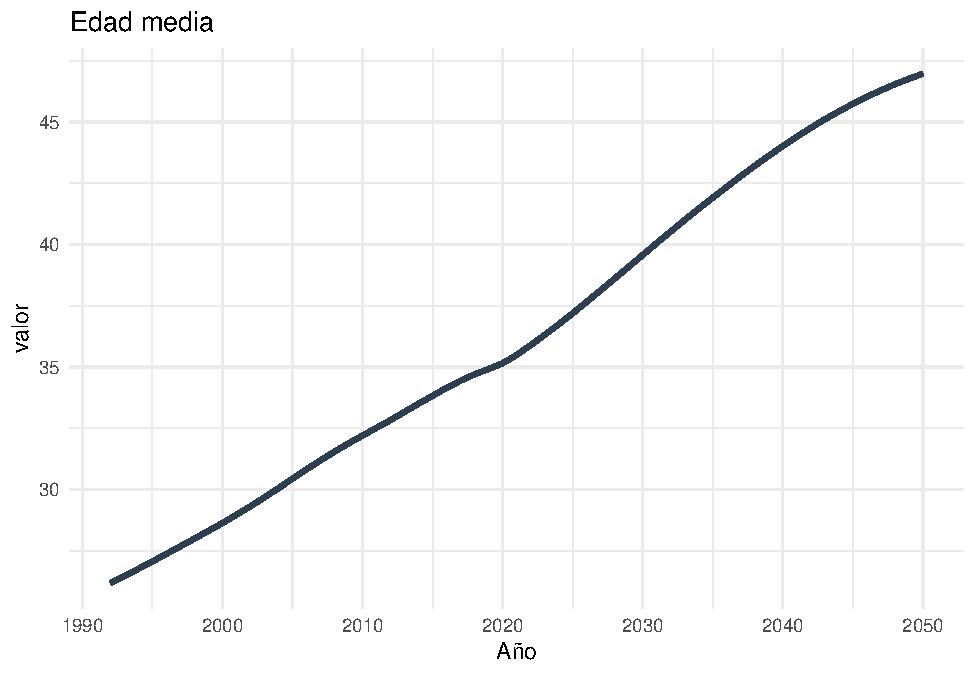
\includegraphics[keepaspectratio]{figs_pdf/edad media-1.pdf}}

\textbf{Análisis descriptivo de la Edad Media de la Población:} Entre
1992 y 2050, la edad media de la población mostró un cambio
significativo, pasando de 26.18 a 46.97 años. Este comportamiento
representa un aumento de 20.79 años en el período considerado. Este
indicador refleja el envejecimiento progresivo de la población, un
factor demográfico clave para evaluar la sostenibilidad de los sistemas
de salud, pensiones y políticas de cuidado a largo plazo, así como para
anticipar cambios en la estructura del mercado laboral.

\pandocbounded{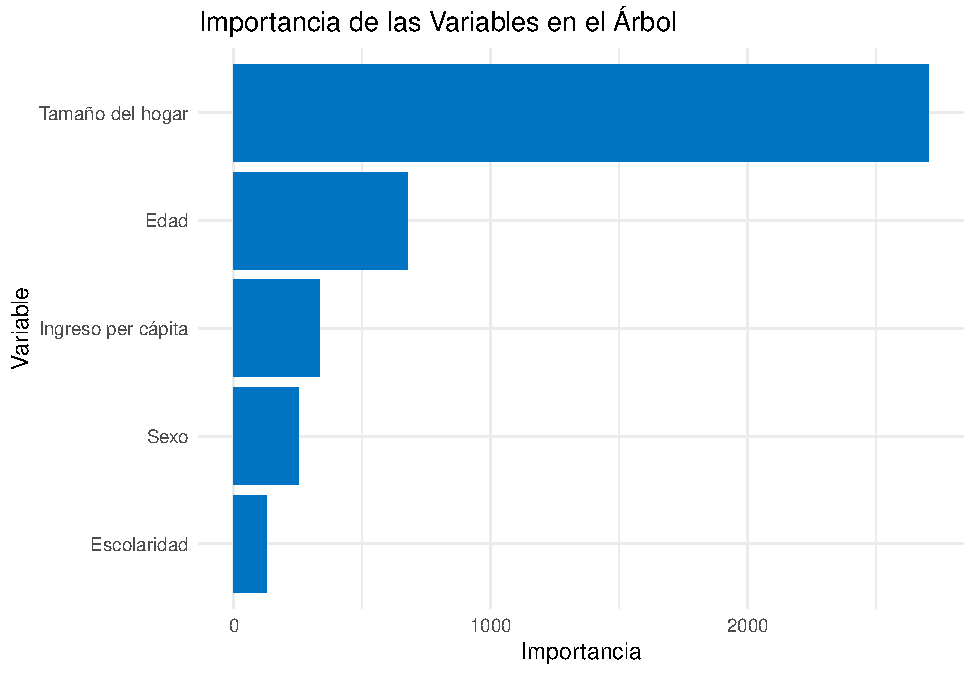
\includegraphics[keepaspectratio]{figs_pdf/unnamed-chunk-2-1.pdf}}

\textbf{Análisis descriptivo del Índice de Envejecimiento:} Según las
proyecciones demográficas basadas en el Censo 2017, el índice de
envejecimiento ha aumentado entre 1992 y 2050, pasando de 21.06 a 176.56
personas mayores de 60 años por cada 100 menores de 15 años. Este
indicador refleja el aumento relativo de la población adulta mayor en
comparación con la población infantil, lo cual tiene implicancias clave
para la planificación de políticas de salud, pensiones y cuidados de
largo plazo.

\pandocbounded{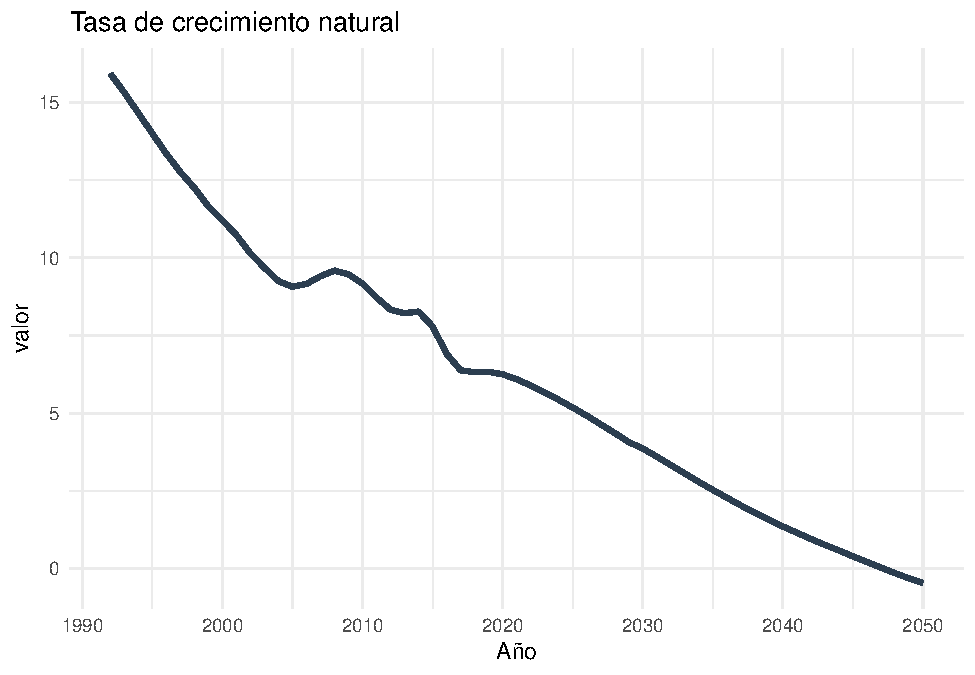
\includegraphics[keepaspectratio]{figs_pdf/unnamed-chunk-4-1.pdf}}

\textbf{Análisis descriptivo de la Tasa de Crecimiento Natural:} Entre
1992 y 2050, la tasa de crecimiento natural ha disminuido, pasando de
15.93 a -0.47 por cada mil habitantes. Este indicador, que representa la
diferencia entre nacimientos y defunciones sin considerar migraciones,
permite visualizar el ritmo de crecimiento poblacional interno del país
y es clave para anticipar dinámicas demográficas como el envejecimiento
o la necesidad de servicios públicos.

\pandocbounded{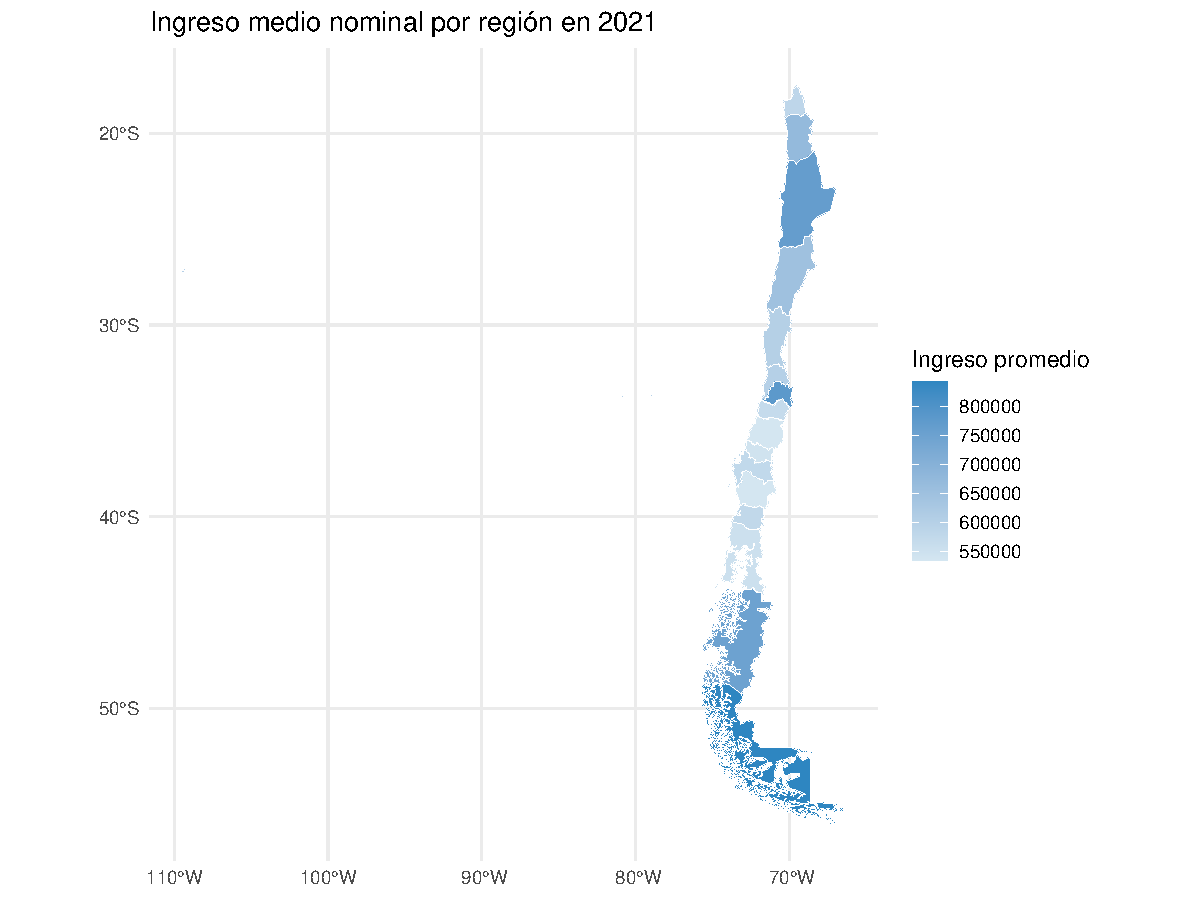
\includegraphics[keepaspectratio]{figs_pdf/mapa_ingreso_2021-1.pdf}}

Entre 2010 y 2021, se observa un incremento generalizado en el ingreso
medio nominal por región. Las regiones con mayor aumento absoluto fueron
Región de Aysén, mientras que el crecimiento más moderado se registró en
Región de O'Higgins. Esta evolución refleja disparidades territoriales
en el ritmo de crecimiento del ingreso.

\begin{center}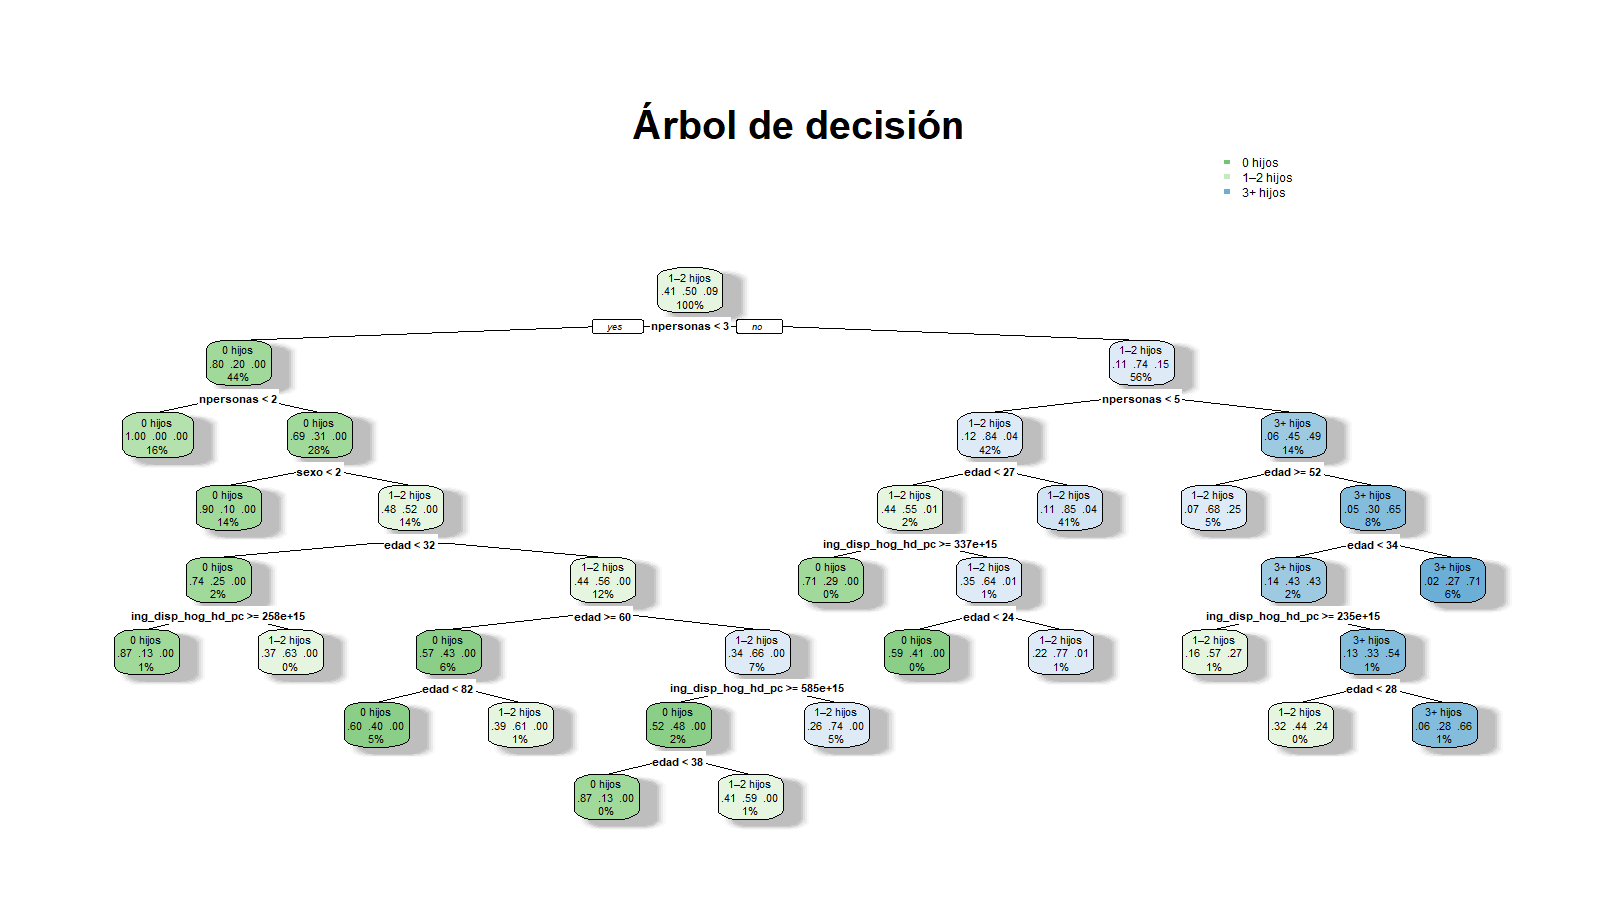
\includegraphics[width=1\linewidth]{figs_pdf/arbol_decision} \end{center}

Se construyó un modelo de árbol de decisión para clasificar a los
hogares según su número de hijos (0, 1--2 o 3 o más). El árbol reveló
que la variable más influyente fue \textbf{Tamaño del hogar}, seguida de
otras variables sociodemográficas relevantes. La variable más influyente
entrega información clave sobre los perfiles familiares. Comprender su
impacto permite segmentar y anticipar dinámicas sociodemográficas.

El modelo alcanzó una precisión global de \textbf{0.829} (IC 95\%: 0.818
-- 0.84) y un coeficiente Kappa de \textbf{0.697}, lo que indica un
desempeño robusto y confiable.

Estos resultados permiten diseñar estrategias segmentadas y basadas en
evidencia, como programas de apoyo a hogares grandes, incentivos a la
planificación familiar o estrategias diferenciadas según perfiles
regionales.

\pandocbounded{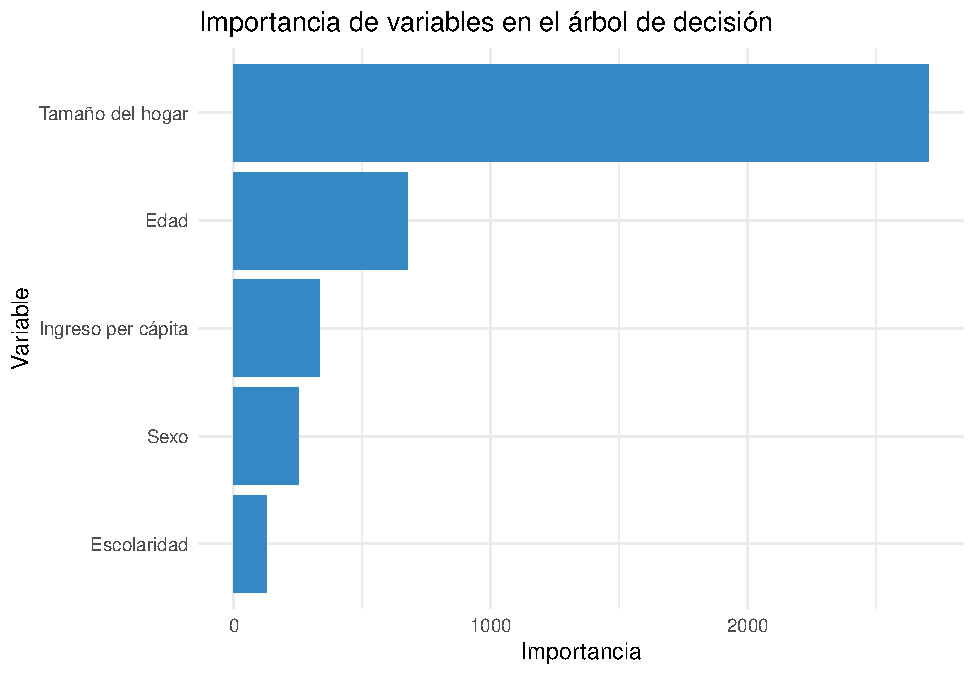
\includegraphics[keepaspectratio]{figs_pdf/unnamed-chunk-10-1.pdf}}

El gráfico anterior presenta la importancia relativa de cada variable
utilizada en el modelo de árbol de decisión. Estas variables contribuyen
de manera diferenciada a predecir el grupo de número de hijos en un
hogar. Las tres variables más influyentes fueron: \textbf{Tamaño del
hogar}, \textbf{Edad} y \textbf{Ingreso per cápita}. Esto implica que
estas características tienen un fuerte poder explicativo para segmentar
a los hogares según su dinámica reproductiva. Por ejemplo, el
\textbf{Tamaño del hogar} tiene un peso considerable en las decisiones
de planificación familiar y en la estructura de los hogares. Estos
hallazgos permiten focalizar políticas públicas o decisiones
estratégicas en los factores más determinantes. El modelo entrega
información procesable para anticipar cambios en la fecundidad y adaptar
iniciativas sociales y económicas con base en evidencia.

\end{document}
